\documentclass[12pt]{article}
\usepackage{geometry}[margin=2cm]
\usepackage{amsmath}
\usepackage{graphicx}
\title{Homework\#3}
\author{Raja Kantheti}
\begin{document}
\maketitle
\section{Problem 14.3}

\subsection*{Part A}

\begin{itemize}
    \item \textbf{Mean:}
    \[
    \text{Mean} = \frac{1}{n} \sum_{i=1}^n x_i = 29.87
    \]
    
    \item \textbf{Median:}
    \[
    \text{Median} = 29.65
    \]
    
    \item \textbf{Mode:}
    \[
    \text{Mode} = 29.65
    \]
    
    \item \textbf{Variance:}
    \[
    \text{Variance} = \frac{1}{n-1} \sum_{i=1}^n \left( x_i - \text{Mean} \right)^2 = 1.41
    \]
    
    \item \textbf{Standard Deviation:}
    \[
    \text{Standard Deviation} = \sqrt{\text{Variance}} = 1.19
    \]
    
    \item \textbf{Mean Absolute Deviation (MAD):}
    \[
    \text{MAD} = \frac{1}{n} \sum_{i=1}^n |x_i - \text{Mean}| = 0.77
    \]
    
    \item \textbf{Coefficient of Variation:}
    \[
    \text{Coefficient of Variation} = \frac{\text{Standard Deviation}}{\text{Mean}} = 0.0398
    \]
\end{itemize}
\subsection*{Part B}

\section{Problem 14.12}
Power law model: $A = 0.415W^{0.380}$\\
Predicted surface area for 95 kg: $2.34 m^2$\\
Prediction interval: $2.31 m^2$ to $2.37 m^2$

Residuals vs Area Plot:

\begin{figure}[h]
    \centering
    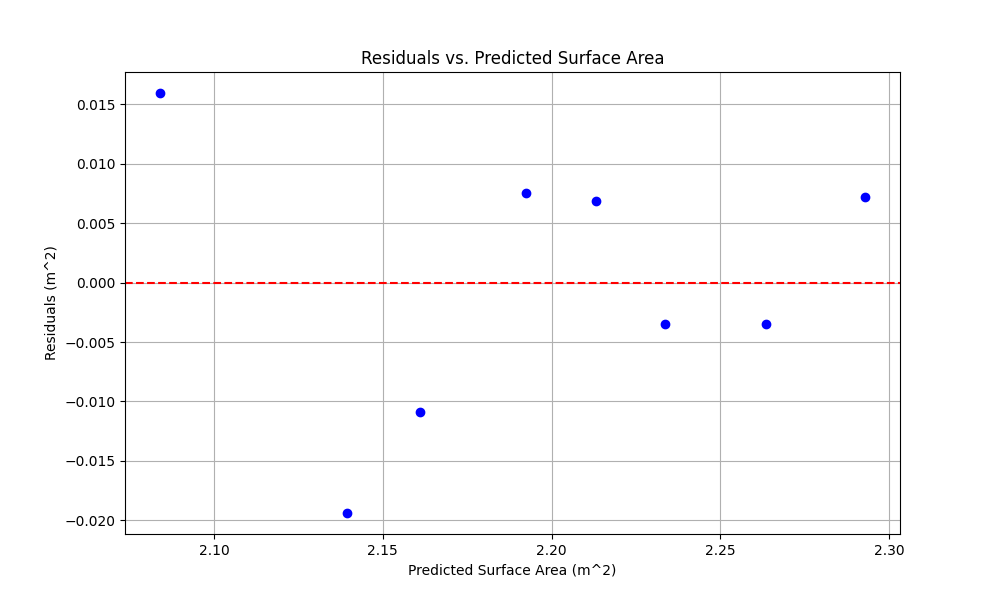
\includegraphics[width=0.5\textwidth]{../residuals_vs_predicted_area.png}
    \caption{Residuals vs Weight}
\end{figure}
Surface area vs Weight plot: 

\begin{figure}[h]
    \centering
    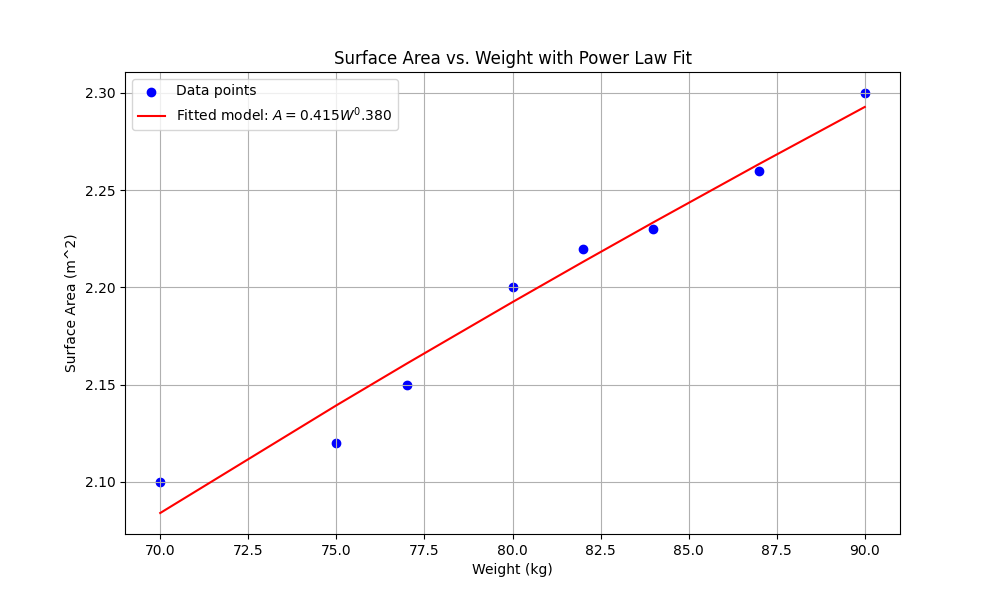
\includegraphics[width=0.5\textwidth]{../surface_area_vs_weight.png}
    \caption{Surface Area vs Weight}
\end{figure}

\section*{15.2}

We are given the model:
\[
y = \beta_1 x + \beta_2 x^2 + \epsilon
\]

where \( y \) is the dependent variable, \( x \) is the independent variable, \(\beta_1\) and \(\beta_2\) are the coefficients we need to estimate, and \(\epsilon\) is the error term.

The objective is to find the values of \(\beta_1\) and \(\beta_2\) that minimize the sum of the squared residuals (the differences between the observed and predicted values of \( y \)).

\subsection*{Least Squares Method}

The least squares method minimizes the sum of the squared residuals:
\[
S = \sum_{i=1}^n \left( y_i - (\beta_1 x_i + \beta_2 x_i^2) \right)^2
\]

\subsection*{Derivation of the Sum of Squared Residuals}

Let's denote the residuals as:
\[
r_i = y_i - (\beta_1 x_i + \beta_2 x_i^2)
\]

Then, the sum of squared residuals is:
\[
S = \sum_{i=1}^n r_i^2 = \sum_{i=1}^n \left( y_i - \beta_1 x_i - \beta_2 x_i^2 \right)^{2}
\]

\subsection*{Minimizing the Sum of Squared Residuals}

taking the partial derivatives of \( S \) with respect to \(\beta_1\) and \(\beta_2\) and set them to zero.

\subsubsection*{Partial Derivative with Respect to \(\beta_1\)}

\[
\frac{\partial S}{\partial \beta_1} = -2 \sum_{i=1}^n x_i \left( y_i - \beta_1 x_i - \beta_2 x_i^2 \right)
\]

Setting this to zero:

\[
\sum_{i=1}^n x_i y_i = \beta_1 \sum_{i=1}^n x_i^2 + \beta_2 \sum_{i=1}^n x_i^3
\]

\subsubsection*{Partial Derivative with Respect to \(\beta_2\)}

\[
\frac{\partial S}{\partial \beta_2} = -2 \sum_{i=1}^n x_i^2 \left( y_i - \beta_1 x_i - \beta_2 x_i^2 \right)
\]

Setting this to zero:

\[
\sum_{i=1}^n x_i^2 y_i = \beta_1 \sum_{i=1}^n x_i^3 + \beta_2 \sum_{i=1}^n x_i^4
\]

\subsection*{Normal Equations}

We now have two normal equations:

1. \[
\sum_{i=1}^n x_i y_i = \beta_1 \sum_{i=1}^n x_i^2 + \beta_2 \sum_{i=1}^n x_i^3
\]

2. \[
\sum_{i=1}^n x_i^2 y_i = \beta_1 \sum_{i=1}^n x_i^3 + \beta_2 \sum_{i=1}^n x_i^4
\]

Matrix Forms of these equations are:

\[
\begin{bmatrix}
\sum x_i^2 & \sum x_i^3 \\
\sum x_i^3 & \sum x_i^4
\end{bmatrix}
\begin{bmatrix}
\beta_1 \\
\beta_2
\end{bmatrix}
=
\begin{bmatrix}
\sum x_i y_i \\
\sum x_i^2 y_i
\end{bmatrix}
\]

These are of the form:

\[
A \beta = b
\]

where:

\[
A = \begin{bmatrix}
\sum x_i^2 & \sum x_i^3 \\
\sum x_i^3 & \sum x_i^4
\end{bmatrix},
\quad
\beta = \begin{bmatrix}
\beta_1 \\
\beta_2
\end{bmatrix},
\quad
b = \begin{bmatrix}
\sum x_i y_i \\
\sum x_i^2 y_i
\end{bmatrix}
\]

To find the coefficients \(\beta_1\) and \(\beta_2\), we solve the system of linear equations \( A \beta = b \).

Mmade a python script to run the calculations and generate the plots. The script is available at: \texttt{test.py}

Here are the values of \(\beta_1\) and \(\beta_2\):
\(beta_1\) = 7.771024464831841\\
\(beta_2\) = 0.11907492354740007

Hrere is the plot of the data and the fitted curve:

\begin{figure}[h]
    \centering
    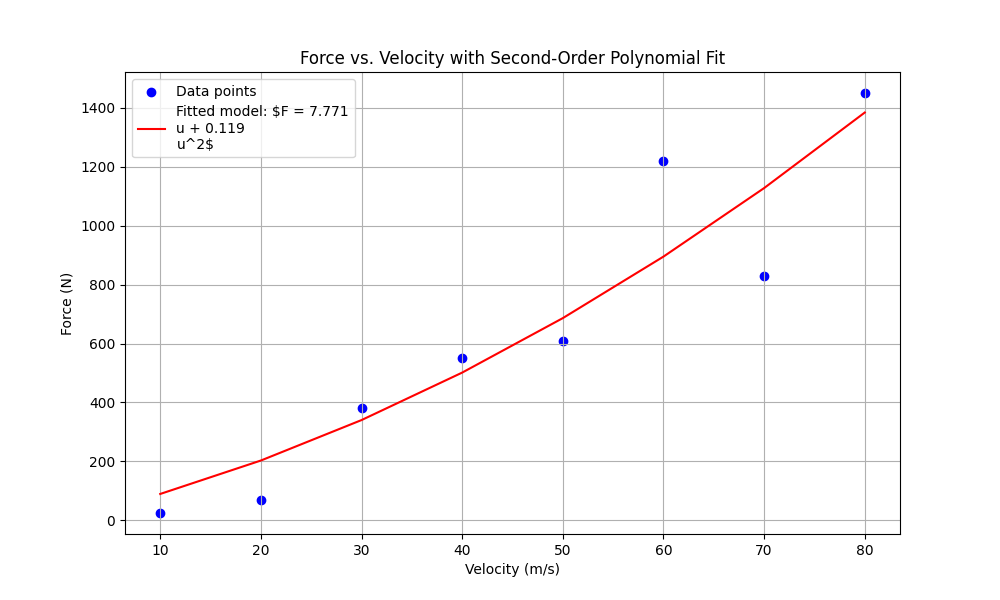
\includegraphics[width=0.5\textwidth]{../force_vs_velocity_fit.png}
    \caption{Data and Fitted Curve}
\end{figure}
\section{16.2}
The temperature in a pond varies sinusoidally over the course of a year. We aim to fit the model:
\[
y = A_0 + A_1 \cos(\omega_0 t) + B_1 \sin(\omega_0 t) + e
\]
to the given data. Using the fitted equation, we will determine the mean, amplitude, and the day and value of the maximum temperature.

Given Data

\[
\begin{array}{c|ccccccccccc}
t \ (\text{days}) & 15 & 45 & 75 & 105 & 135 & 165 & 225 & 255 & 285 & 315 & 345 \\
\hline
T \ (C) & 3.4 & 4.7 & 8.5 & 11.7 & 16 & 18.7 & 19.7 & 17.1 & 12.7 & 7.7 & 5.1 \\
\end{array}
\]

Determine \(\omega_0\)

Since the period is 365 days, the angular frequency \(\omega_0\) is:

\[
\omega_0 = \frac{2\pi}{365} \approx 0.0172 \text{ rad/day}
\]

Design Matrix

For each given day \( t \)  \( \cos(\omega_0 t) \) and \( \sin(\omega_0 t) \) are as sfollows: 

\[
\begin{array}{c|ccccccccccc}
t \ (\text{days}) & 15 & 45 & 75 & 105 & 135 & 165 & 225 & 255 & 285 & 315 & 345 \\
\hline
\cos(\omega_0 t) & 0.967 & 0.716 & 0.275 & -0.230 & -0.667 & -0.954 & -0.721 & -0.309 & 0.204 & 0.646 & 0.946 \\
\sin(\omega_0 t) & 0.255 & 0.697 & 0.961 & 0.973 & 0.745 & 0.299 & -0.693 & -0.951 & -0.979 & -0.763 & -0.329 \\
\end{array}
\]

Calculate the Necessary Sums

\[
\begin{aligned}
\sum \cos(\omega_0 t) &= 0.173 \\
\sum \sin(\omega_0 t) &= 0.215 \\
\sum \cos^2(\omega_0 t) &= 5.927 \\
\sum \sin^2(\omega_0 t) &= 4.073 \\
\sum \cos(\omega_0 t) \sin(\omega_0 t) &= -0.218 \\
\sum T &= 125.3 \\
\sum T \cos(\omega_0 t) &= -3.075 \\
\sum T \sin(\omega_0 t) &= 4.338 \\
\end{aligned}
\]


Using the sums calculated, we set up the normal equations:

\[
\begin{bmatrix}
11 & 0.173 & 0.215 \\
0.173 & 5.927 & -0.218 \\
0.215 & -0.218 & 4.073 \\
\end{bmatrix} \begin{bmatrix}
A_0 \\
A_1 \\
B_1 \\
\end{bmatrix} = \begin{bmatrix}
125.3 \\
-3.075 \\
4.338 \\
\end{bmatrix}
\]

Usedd the python sccript to solve the normal equations and calculate the coefficients. The script is available at: \texttt{test.py}\\
The plot shows the equation fits the data well. 

\begin{figure}[h]
    \centering
    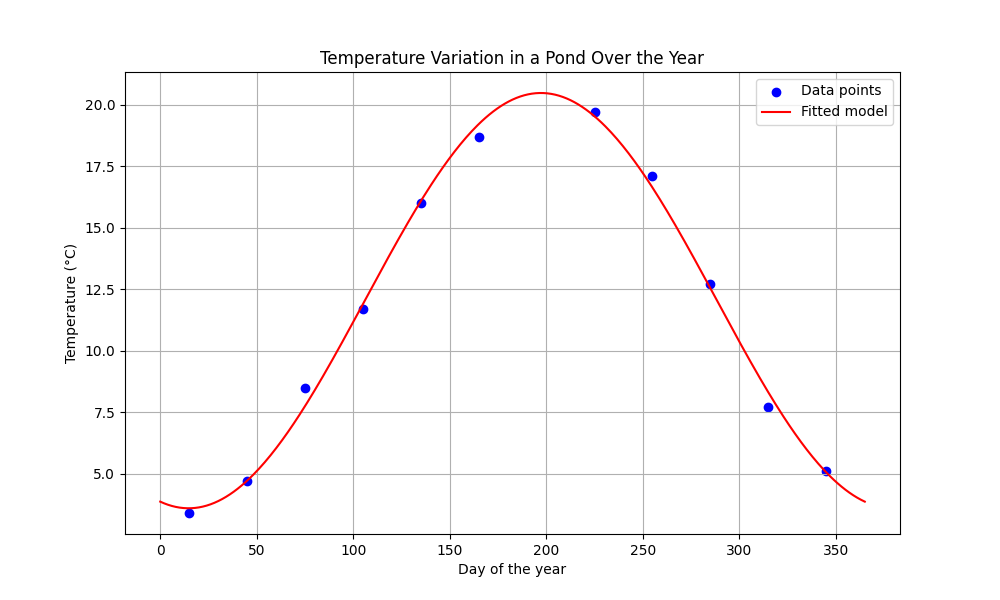
\includegraphics[width=0.5\textwidth]{../temperature_fit.png}
    \caption{Data and Fitted Curve}
\end{figure}
\section{17.2}
Given Data,
\[
\begin{array}{c|ccccccc}
x & 0 & 1 & 2.5 & 3 & 4.5 & 5 & 6 \\
\hline
y & 2 & 5.4375 & 7.3516 & 7.5625 & 8.4453 & 9.1875 & 12 \\
\end{array}
\]

\section*{Selected Points Around \( x = 3.5 \)}

\[
\begin{array}{c|cccc}
x & 2.5 & 3 & 4.5 & 5 \\
\hline
y & 7.3516 & 7.5625 & 8.4453 & 9.1875 \\
\end{array}
\]

\section*{Finite Divided Differences}

1. First-order divided differences:

\[
f[x_i, x_{i+1}] = \frac{f(x_{i+1}) - f(x_i)}{x_{i+1} - x_i}
\]

\[
\begin{aligned}
f[2.5, 3] &= \frac{7.5625 - 7.3516}{3 - 2.5} = \frac{0.2109}{0.5} = 0.4218 \\
f[3, 4.5] &= \frac{8.4453 - 7.5625}{4.5 - 3} = \frac{0.8828}{1.5} = 0.5885 \\
f[4.5, 5] &= \frac{9.1875 - 8.4453}{5 - 4.5} = \frac{0.7422}{0.5} = 1.4844 \\
\end{aligned}
\]

2. Second-order divided differences:

\[
f[x_i, x_{i+1}, x_{i+2}] = \frac{f[x_{i+1}, x_{i+2}] - f[x_i, x_{i+1}]}{x_{i+2} - x_i}
\]

\[
\begin{aligned}
f[2.5, 3, 4.5] &= \frac{0.5885 - 0.4218}{4.5 - 2.5} = \frac{0.1667}{2} = 0.08335 \\
f[3, 4.5, 5] &= \frac{1.4844 - 0.5885}{5 - 3} = \frac{0.8959}{2} = 0.44795 \\
\end{aligned}
\]

3. Third-order divided differences:

\[
f[x_i, x_{i+1}, x_{i+2}, x_{i+3}] = \frac{f[x_{i+1}, x_{i+2}, x_{i+3}] - f[x_i, x_{i+1}, x_{i+2}]}{x_{i+3} - x_i}
\]

\[
\begin{aligned}
f[2.5, 3, 4.5, 5] &= \frac{0.44795 - 0.08335}{5 - 2.5} = \frac{0.3646}{2.5} = 0.14584 \\
\end{aligned}
\]

\section*{Newton Interpolating Polynomial}

The Newton interpolating polynomial is given by:

\[
P(x) = f[x_0] + f[x_0, x_1](x - x_0) + f[x_0, x_1, x_2](x - x_0)(x - x_1) + f[x_0, x_1, x_2, x_3](x - x_0)(x - x_1)(x - x_2)
\]

Using the points \((2.5, 7.3516)\), \((3, 7.5625)\), \((4.5, 8.4453)\), and \((5, 9.1875)\):

\[
\begin{aligned}
P(x) &= 7.3516 + 0.4218(x - 2.5) + 0.08335(x - 2.5)(x - 3) + 0.14584(x - 2.5)(x - 3)(x - 4.5) \\
\end{aligned}
\]

\section*{Evaluate the Polynomial at \( x = 3.5 \)}

\[
\begin{aligned}
P(3.5) &= 7.3516 + 0.4218(3.5 - 2.5) + 0.08335(3.5 - 2.5)(3.5 - 3) + 0.14584(3.5 - 2.5)(3.5 - 3)(3.5 - 4.5) \\
       &= 7.3516 + 0.4218(1) + 0.08335(1)(0.5) + 0.14584(1)(0.5)(-1) \\
       &= 7.3516 + 0.4218 + 0.041675 - 0.07292 \\
       &= 7.742155 - 0.07292 \\
       &= 7.669235 \\
\end{aligned}
\]

So, estimated value of \( y \) at \( x = 3.5 \) is approximately \( 7.6692 \).

\end{document}